\documentclass{article}
\usepackage[utf8]{inputenc}
\usepackage[spanish]{babel}
\usepackage{graphicx, graphics, float, fancyhdr, titling}
\usepackage{listings}
\usepackage[a4paper, total={6in, 9.5in}]{geometry}
\usepackage{fancyhdr}
\usepackage{hyperref}   %para que funcione addcontentsline debe ser la ultima que se cargue

%\setcounter{secnumdepth}{-2}       %Poner solo esto si no se quieren numero delante de las secciones y niveles inferiores.

\renewcommand{\footrulewidth}{0.4pt}
\title{

\includegraphics[width=1.75in]{imagenes/UGR-Logo.png} \\
\vspace*{1in}
\textbf{Cuestiones Tema 2} \\
Animación por Ordenador \\
\vspace*{0.5in}}
\author{Andrés Merlo Trujillo \\
andresmerlo@correo.ugr.es \\
77147239H \\ 
\vspace*{0.5in} \\
E.T.S. de Ingenierías Informática y de Telecomunicación \\
\textbf{Universidad de Granada}} \date{\today}

\hypersetup{
    colorlinks=true,
    linkcolor=black,
    citecolor=black
}

\renewcommand\maketitlehooka{\null\mbox{}\vfill}
\renewcommand\maketitlehookd{\vfill\null}

\begin{document}
\begin{titlingpage}
\maketitle
\end{titlingpage}

\tableofcontents

\newpage

\pagestyle{fancy}   %a partir de comienza el header (se salta el indice y portada)
\fancyhead[L]{Andrés Merlo Trujillo}
\fancyhead[R]{Animación por Ordenador}
%\section{Ejercicio 1}
%\begin{figure}[H]
%    \centering
%    \includegraphics[width=\textwidth]{imagenes/passwdfile.png}
%\end{figure}

\section{Busca el resto de principios de animación, descríbelos brevemente e indica un ejemplo visual de cada uno.}

Voy a explicar cada uno de los principios en subsecciones a continuación.

% overlap: meh
% slow: arreglar forma en que se dicen las cosas (esta muy raro escrito)
\subsection{Overlap \& Follow Through}

Son dos técnicas que se utilizan con el objetivo de crear una animación más realista y para dar la sensación de que el personaje tiene una inercia \cite{overlap}. La idea principal de estas técnicas las partes secundarias de un personaje se mueven a un ritmo diferente del personaje durante el movimiento del mismo y mantienen algo de inercia cuando el personaje se para.

\bigskip

\textit{Follow Through} se basa en la idea de que ciertas partes conectadas a un personaje/objeto se seguirán moviendo después de que dicho objeto haya parado \cite{overlap}.

\bigskip

Mientras que el \textit{Overlapping} se fundamenta en que las partes conectadas a un personaje/objeto se moverán a un ritmo diferente del mismo \cite{overlap}, normalmente en el sentido contrario en el que se mueve dicho personaje, para dar sensación de velocidad.

\bigskip

Ejemplos de este principio pueden ser: movimientos de brazos de un personaje, movimiento de las orejas de un animal que corre y luego para, o incluso el movimiento de antenas de un personaje.

\begin{figure}[H]
    \centering
    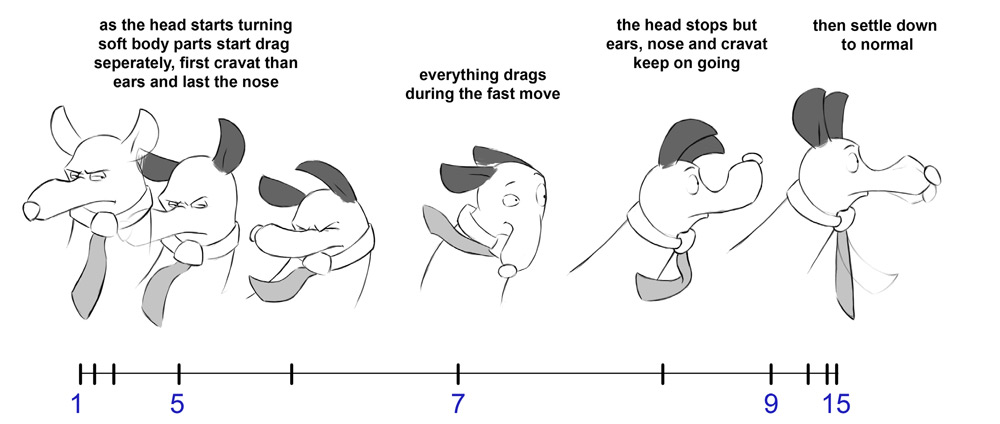
\includegraphics[width=\textwidth]{imagenes/overlap-08.jpg}
    \caption{Ejemplo del principio de \textit{Overlapping} y \textit{Follow Through}. Se puede ver en las orejas y la corbata.}
    \vspace{10pt}
    \footnotesize{Fuente: \url{https://www.robert-kuczera.de/3d-character-animation-tutorial-secondary-actoin.html}}
\end{figure}

\subsection{Slow-in \& Slow-out}

Este principio consiste en hacer que un objeto acelere cuando vaya a comenzar a moverse y decelere cuando se vaya a parar. En la vida real, los objetos no se mueven sin antes acelerar o desacelerar, por lo que omitir este principio en una animación puede hacer que los movimientos parezcan poco naturales, robóticos y abruptos. \cite{plural}

\bigskip

Un ejemplo de este principio es el de un coche que comienza parado, para después llegar a una velocidad y finalmente detenerse de nuevo. El coche necesita un tiempo para llegar a la velocidad deseada; es decir, una aceleración. Luego cuando frena pasa exactamente lo mismo, no para bruscamente, sino que va desacelerando poco a poco. \cite{plural}

\bigskip

En animación tradicional, esto se realiza utilizando la técnica de espaciados. Al principio y al final de la animación se añaden más fotogramas consecutivos, para dar la sensación de que el objeto se arranca y detiene gradualmente. Mientras que el espaciado es constante en el resto de la animación, haciendo que su velocidad sea también constante.

\bigskip

En animación por ordenador, normalmente se utiliza una curva \textit{Ease-In/Ease-Out}, cuyo resultado es el mismo que empleando las técnicas mencionadas anteriormente para las animaciones tradicionales, pero requiriendo menos esfuerzo y de manera automática.

\begin{figure}[H]
    \centering
    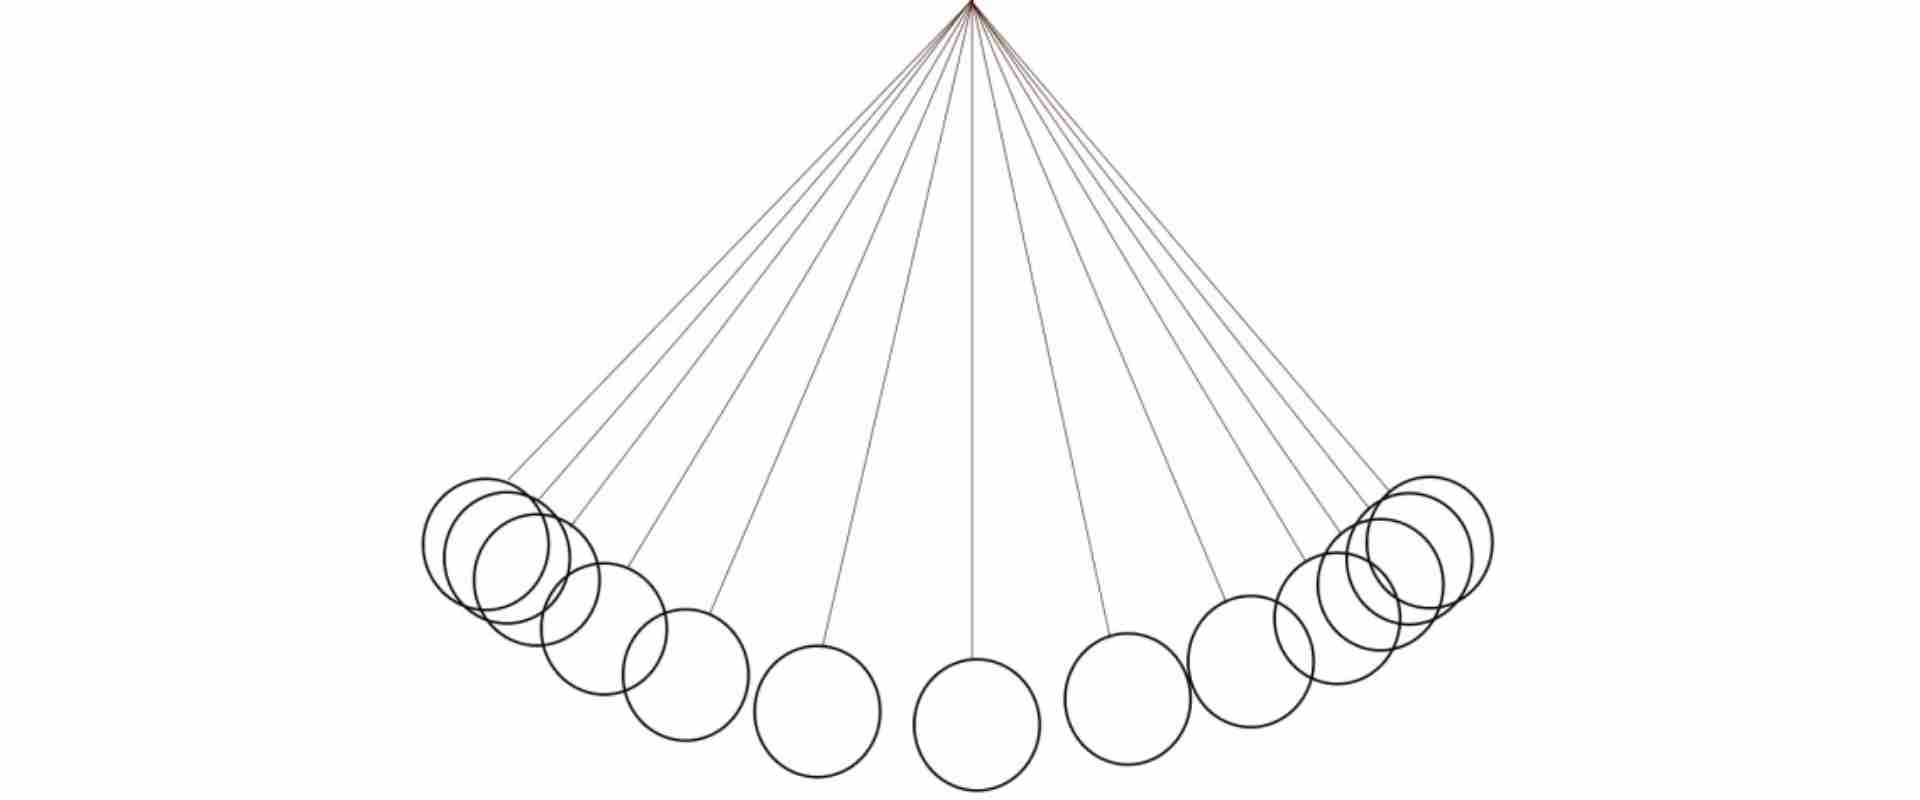
\includegraphics[width=\textwidth]{imagenes/Slow-In-and-Slow-Out.jpg}
    \caption{Ejemplo del principio \textit{Slow-In \& Slow-Out}. Se puede ver como el péndulo en los extremos acelera y desacelera mediante el espaciado de los fotogramas.}
    \vspace{10pt}
    \footnotesize{Fuente: \url{https://darvideo.tv/dictionary/slow-in-slow-out/}}
\end{figure}

\subsection{Arcos}

% En la vida real, gran parte de los movimientos y acciones que ocurren siguen una trayectoria circular, conocida como arco \cite{arcsdsource}. Estos arcos se pueden producir porque incide más de una fuerza en el objeto, haciendo que este se mueva trazando un arco \cite{arcslinkedin}. Otro motivo es porque existen objetos que poseen un pivote (como un brazo), haciendo que el movimiento que realicen se restrinja al arco.

En la vida real, gran parte de los movimientos y acciones que ocurren siguen una trayectoria circular, conocida como arco \cite{arcsdsource}. Estos arcos pueden ser el resultado de más de una fuerza actuando sobre un objeto, haciendo que se mueva trazando una trayectoria curva (arco) \cite{arcslinkedin}. Otro motivo es porque hay objetos que tienen un pivote, como puede ser un brazo, lo que restringe el movimiento a un arco.

\bigskip

Utilizar arcos hace que la animación sea más natural y fluida, haciendo que sea más creíble para el espectador. Si no se aplicase este principio, la animación sería demasiado mecanizada y robótica.

\bigskip

Algunos ejemplos que se pueden beneficiar de los arcos son: rebote de una pelota, movimiento de una extremidad de un personaje y el movimiento de una rama por el viento.

\begin{figure}[H]
    \centering
    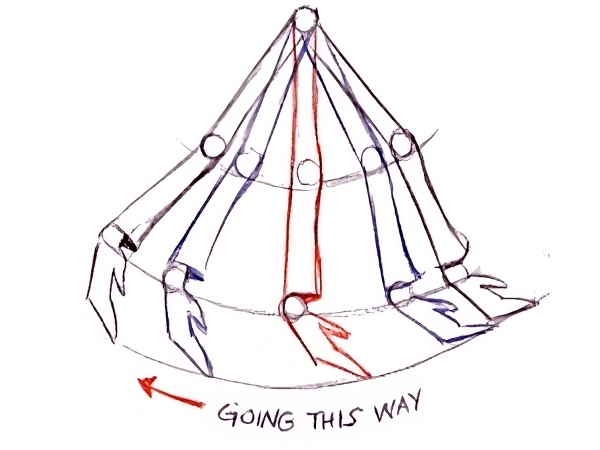
\includegraphics[width=\textwidth]{imagenes/arm-arc.jpg}
    \caption{Ejemplo del principio Arcos. Se puede ver como el movimiento del brazo sigue un arco.}
    \vspace{10pt}
    \footnotesize{Fuente: \url{https://johnhannonblog.wordpress.com/2015/12/01/12-principles-of-animation-arc/}}
\end{figure}

\begin{figure}[H]
    \centering
    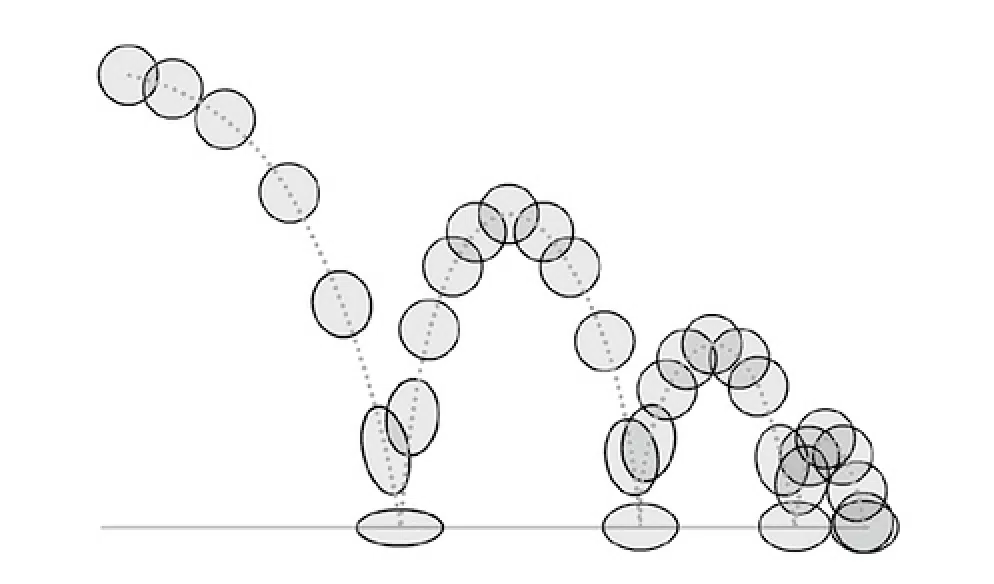
\includegraphics[width=\textwidth]{imagenes/bouncing-ball.png}
    \caption{Otro ejemplo de Arcos. La fuerza de la gravedad y la de lanzamiento se combinan para crear un arco.}
    \vspace{10pt}
    \footnotesize{Fuente: \url{https://idearocketanimation.com/13721-12-principles-of-animation-gifs/}}
\end{figure}

\subsection{Acción secundaria}

Consiste en las acciones que enfatizan la acción principal para darle mas vida a la animacion y hacer que las acciones del personaje sean mas convincentes. Debe ser algo sutil, que no distraiga o tape la accion principal, ya que solo debe aportar mas expresividad a la principal. \cite{plural}

\bigskip

Además, permite mostrar de manera subconsciente lo que el personaje está pensando \cite{idearocket}, como su estado de ánimo.

\bigskip

Un ejemplo de esto es alguien esperando (acción principal) en una sala de espera, si se le añade la acción secundaria de estar dadndo toques con el pie repetidamente, se percibe la sensación de que está esperando nervioso.

\begin{figure}[H]
    \centering
    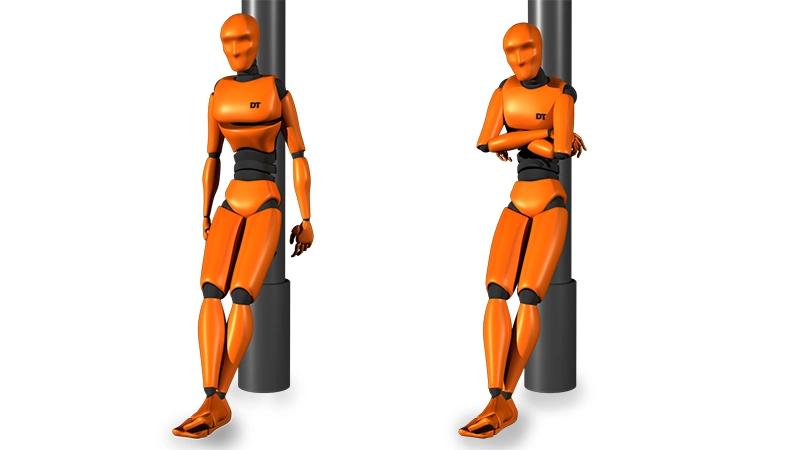
\includegraphics[width=\textwidth]{imagenes/secondary-action.png}
    \caption{Ejemplo de acción secundaria. Se puede ver que puede transmitir otra sensación la posición de los brazos.}
    \vspace{10pt}
    \footnotesize{Fuente: \url{https://www.pluralsight.com/blog/film-games/understanding-12-principles-animation}}
\end{figure}


\begin{figure}[H]
    \centering
    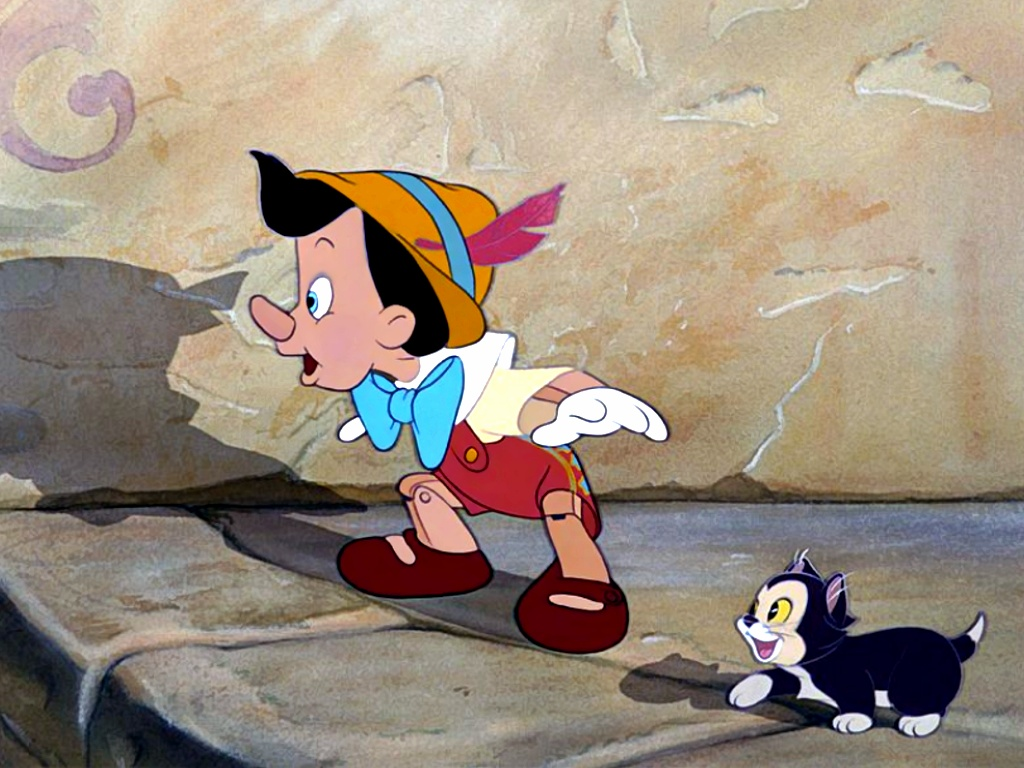
\includegraphics[width=\textwidth]{imagenes/sec-ac.jpg}
    \caption{Otro ejemplo de acción secundaria. Se puede ver que la expresión facial se complementa con los brazos levantados.}
    \vspace{10pt}
    \footnotesize{Fuente: \url{https://animation2012.weebly.com/secondary-action.html}}
\end{figure}
\subsection{Timing}

Consiste en como distribuir los fotogramas de una acción; es decir, en cuantos fotogramas se debe realizar una acción \cite{idearocket}.

\bigskip

El \textit{timing} se puede aplicar a velocidad de movimientos o la duración de los fotogramas. Ajustando el \textit{timing}, se puede expresar que un personaje es más ágil o pesado, más rápido o más lento, etc. También permite mostrar sitaciones de nerviosismo, comeddia, etc.

\bigskip

Un ejemplo de esto puede ser para escenas en películas de acción, donde el personaje necesita actuar rápido para poder alcanzar un objetivo. En este caso lo mejor es usar un timing más espaciado, haciendo menos fotogramas para dar la sensación de rapidez en la escena. 
%dejado intencionadamente asi
Otro ejemplo puede ser el de un espectador en una pista de carreras observando los coches, estos deben tener pocos fotogramas para dar la sensación de que va muy rápido.

\begin{figure}[H]
    \centering
    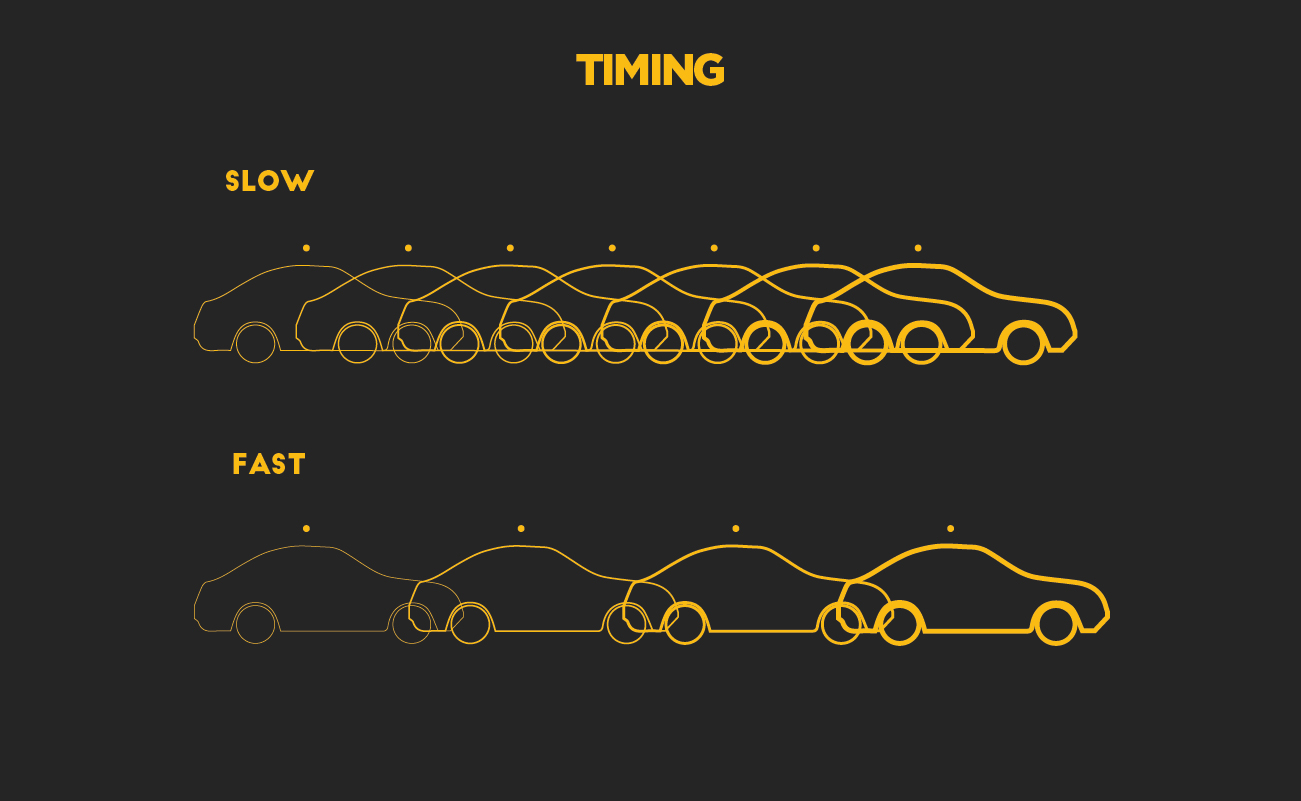
\includegraphics[width=\textwidth]{imagenes/image-9_timing.jpg}
    \caption{Ejemplo de \textit{timing}.}
    \vspace{10pt}
    \footnotesize{Fuente: \url{https://www.360south.com.au/blog/article/27/the-12-principles-of-animation-part-three.html}}
\end{figure}

\subsection{Exageración}

Consiste en exagerar los movimientos, emociones y acciones de los personajes con el objetivo de que la animación sea más humorística, emocionante o dramática.

\bigskip

Un ejemplo clásico es el de un personaje sorprendido, ya que normalmente los animadores lo dibujan con los ojos mucho más abiertos de lo normal (e incluso en algunos casos se puedan salir) y su boca se abra de par en par.

\begin{figure}[H]
    \centering
    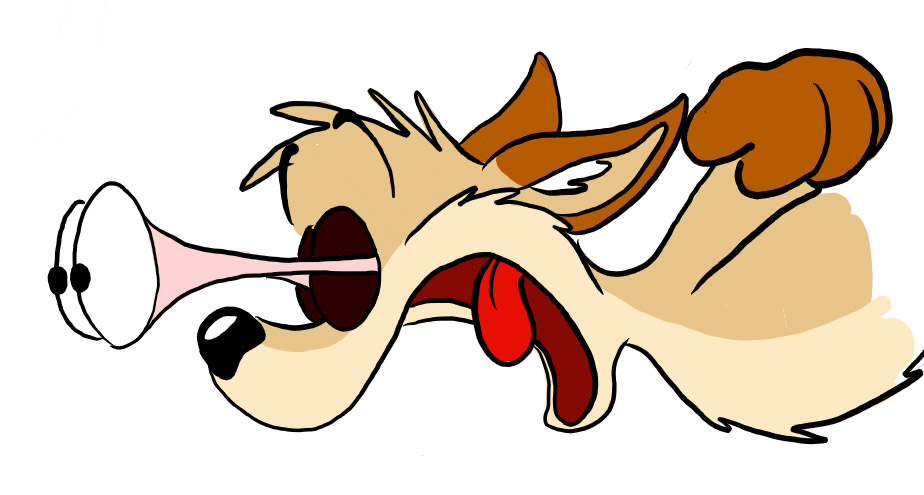
\includegraphics[width=\textwidth]{imagenes/080104_eyes.jpg}
    \caption{Ejemplo de exageracion.}
    \vspace{10pt}
    \footnotesize{Fuente: \url{https://nutchelleblog.wordpress.com/2015/11/22/exaggeration/}}
\end{figure}

\begin{figure}[H]
    \centering
    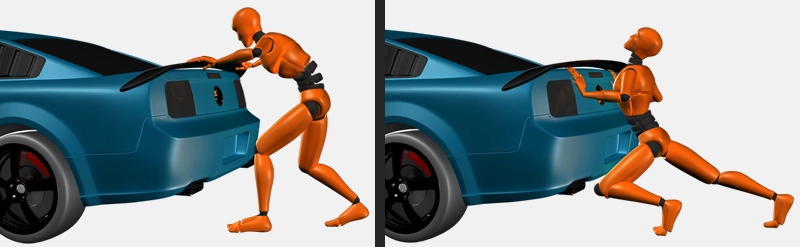
\includegraphics[width=\textwidth]{imagenes/Exaggeration.png}
    \caption{Otro ejemplo de exageracion mas realista.}
    \vspace{10pt}
    \footnotesize{Fuente: \url{https://www.pluralsight.com/blog/film-games/understanding-12-principles-animation}}
\end{figure}

\subsection{Poses sólidas}

Se refiere a la habilidad de crear dibujos tridimensionales que tengan una sensacion de peso, profundidad y volumen correctos y convicentes \cite{plural}.

\bigskip

Es esencial que los animadores tengan una clara comprensión del espacio tridimensional y perspectivas de todos los ángulos de los personajes para poder ubicar los objetos de manera correcta en el espacio y tenga la escena sensación de profundidad.

\bigskip

Otro aspecto importante de las poses sólidas es el de evitar \textit{twinning}, que como se dijo en clase, consiste en evitar poner cualquier par de extremidades simétricas, ya que resulta muy forzado y rígido \cite{plural}.

\begin{figure}[H]
    \centering
    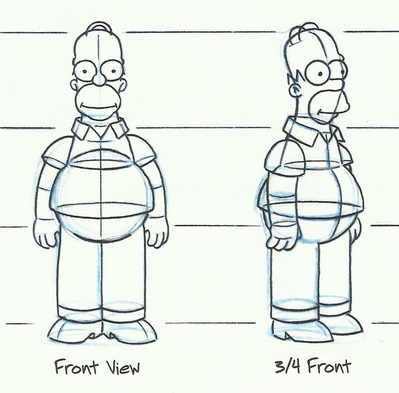
\includegraphics[width=\textwidth]{imagenes/homer-solid-drawing.jpg}
    \caption{Ejemplo de poses sólidas. Aparece Homer en diferentes perspectivas correctamente. También es un buen ejemplo de \textit{twinning}, es demasiado rígido al ser simétrico.}
    \vspace{10pt}
    \footnotesize{Fuente: \url{https://johnhannonblog.wordpress.com/2015/12/01/12-principles-of-animation-solid-drawing/}}
\end{figure}

\subsection{Personalidad}

Se basa en la idea de crear personajes atractivos (en el sentido de que sean agradables a la vista) y carismáticos, incluyendo incluso los antagonistas. Esto hace que sean más fáciles de recordar, más interesantes para el espectador e incluso puede hacer que tengan conexión emocional con un personaje. \cite{idearocket}

\bigskip

La forma más común es caricaturizando a los personajes; es decir, agrandar los rasgos más importantes de la cara e incluso cambiarles la forma del cuerpo para resaltar su estado físico.


\begin{figure}[H]
    \centering
    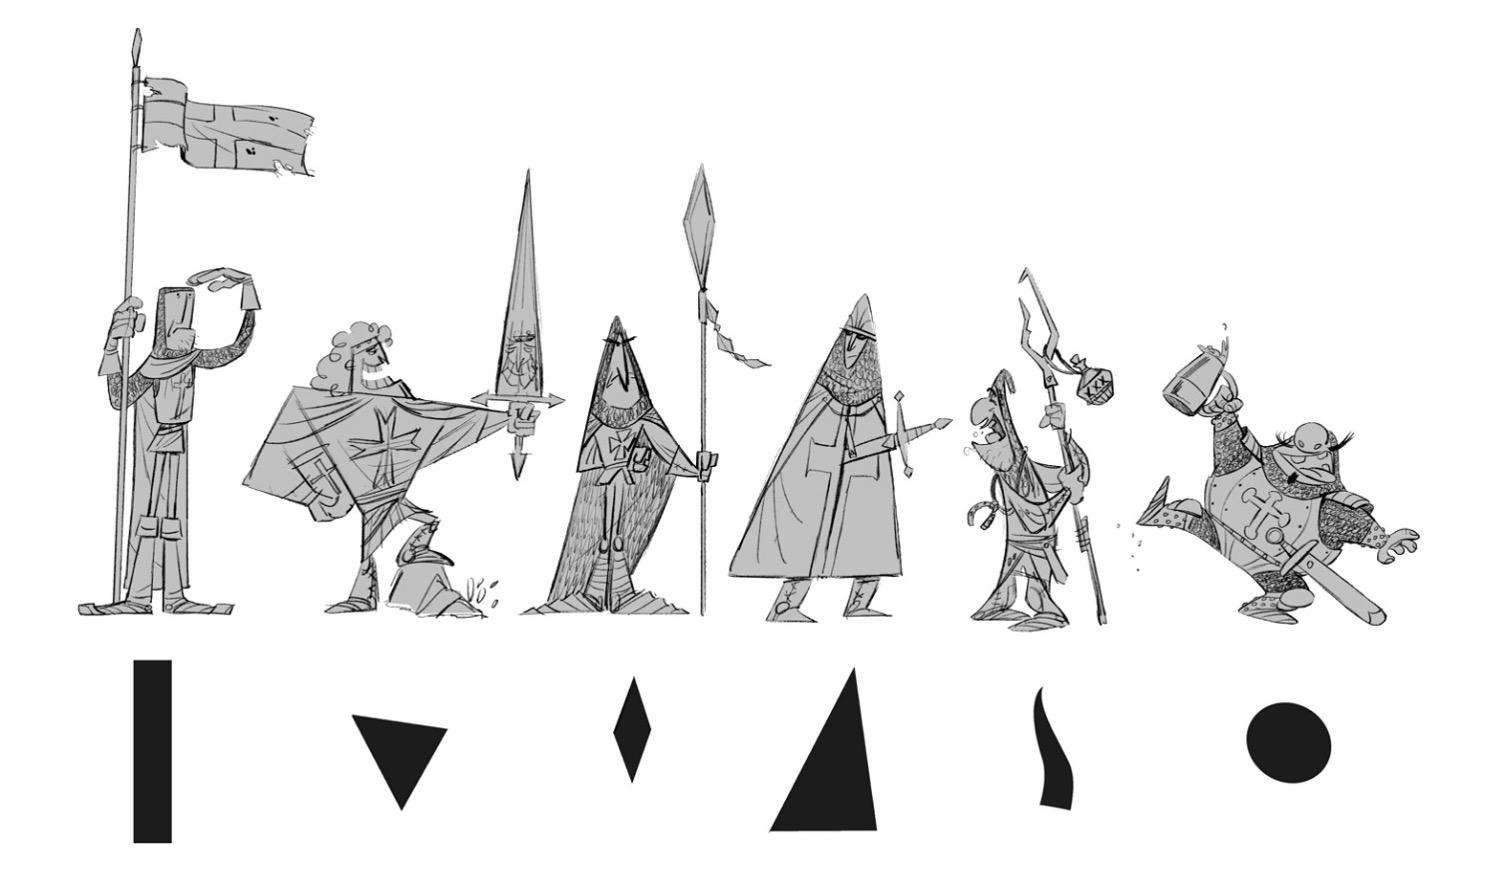
\includegraphics[width=\textwidth]{imagenes/appeal.jpg}
    \caption{Personajes basados en distintas formas para que tengan más personalidad.}
    \vspace{10pt}
    \footnotesize{Fuente: \url{https://www.kdanmobile.com/en/animation-desk/education/animation-principle-character-design}}
\end{figure}

\section{Usando 3DS Max, aplica la técnica de Slow-in \& Slow-out para conseguir los siguientes efectos y justifica en qué momento se está aplicando cada uno}

Para realizar la prueba, he animado una esfera para que se mueva en la escena y he abierto el editor de curvas para observar la curva resultante. Cabe destacar que 3ds Max por defecto anima usando Slow-in/Slow-out, por lo que no ha sido necesario modificar la forma de la curva, solo he modificado un poco la forma para que la aceleracion y el frenado sean mas pronunciados.

\bigskip

La curva resultante de la animación es la siguiente:

\begin{figure}[H]
    \centering
    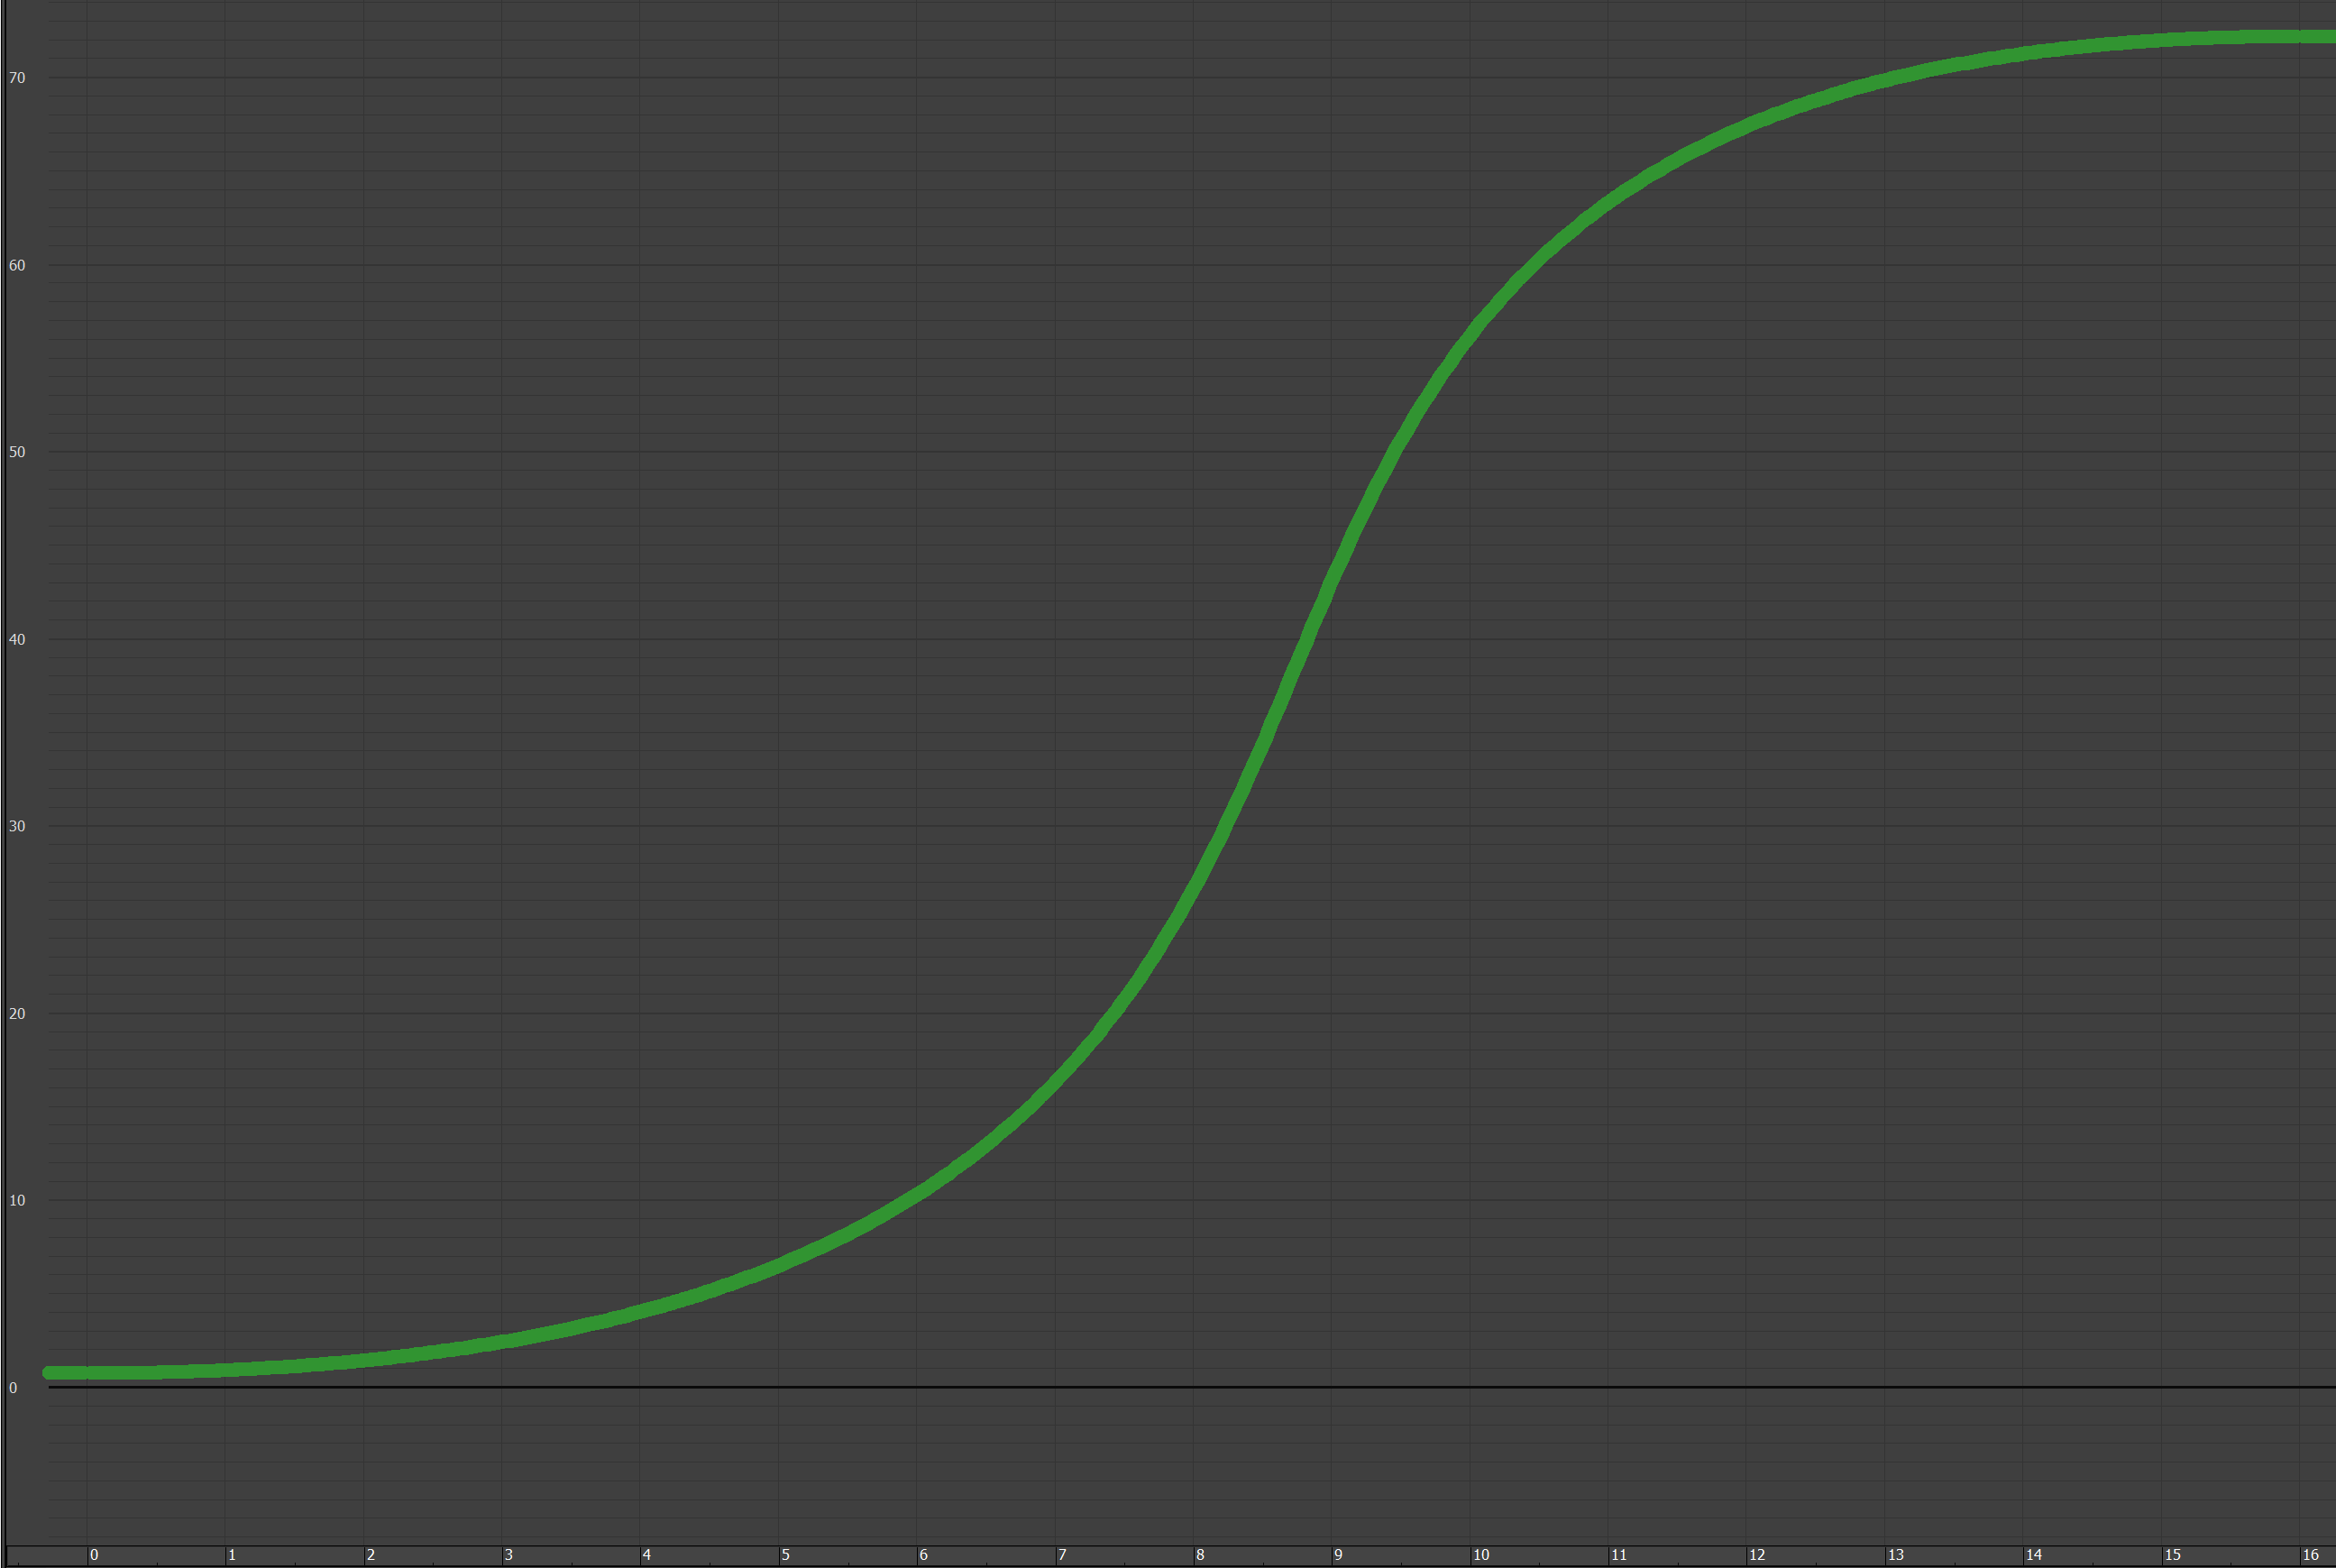
\includegraphics[width=\textwidth]{imagenes/curva.png}
    \caption{Curva de animación para la esfera.}
\end{figure}

El eje X de la gráfica representa el tiempo transcurrido, mientras que el eje Y representa la posición/rotación/escalado del objeto (en este caso translacion en el eje Y).

\subsection{Aceleración desde una pose}
La aceleración desde una pose (en este caso el movimiento de la esfera) se realiza al principio de la animación porque la pendiente de la función comienza a ser mayor, haciendo que cada vez recorra más distancia en la misma cantidad de tiempo.
\subsection{Deceleración hacia una pose}

La deceleración se realiza justo antes de que acabe la animación, ya que es el caso contrario al anterior; es decir, la pendiente de la función se va haciendo menor conforme se acerca al \textit{keyframe}, haciendo que recorra cada vez menos distancia por unidad de tiempo.


\begin{thebibliography}{1}
    \bibitem{overlap} Definición de \textit{Overlapping y Follow Through}: \url{https://www.brownbagfilms.com/labs/entry/12-principles-of-animation-follow-through-and-overlapping-action-tutorials} 
    \bibitem{plural} Definición de \textit{Slow-in \& Slow-out}, acciones secundarias y poses sólidas. Inlcuyendo ejemplos para \textit{Slow-in \& Slow-out}: \url{https://www.pluralsight.com/blog/film-games/understanding-12-principles-animation}
    \bibitem{arcsdsource} Parte de la definición de Arcos: \url{https://dsource.in/course/principles-animation/arcs}
    \bibitem{arcslinkedin} Continuación de la definición de Arcos: \url{https://es.linkedin.com/learning/fundamentos-de-la-animacion/arcos-de-la-animacion}
    \bibitem{idearocket} Definiciones de Acción secundaria, \textit{Timing} y Personalidad: \url{https://idearocketanimation.com/13721-12-principles-of-animation-gifs/}
\end{thebibliography}
\end{document}
